\documentclass[journal,12pt,onecolumn]{IEEEtran}
\usepackage{graphicx, float}
\graphicspath{{Figs/}}
\usepackage{multicol}
\usepackage{parskip}
\usepackage{titlesec}
\usepackage{color}
\usepackage{enumitem}
\usepackage{amsmath,amssymb,amsfonts,amsthm}
\usepackage{array}
\usepackage{booktabs}
\usepackage[table]{xcolor}
\usepackage{longtable}
\usepackage{gensymb}
\usepackage{cite}
\usepackage{algorithmic}
\usepackage{textcomp}
\usepackage{txfonts}
\usepackage{listings}
\usepackage{mathtools}
\usepackage{comment}
\usepackage{tkz-euclide}
\usepackage[breaklinks=true]{hyperref}
\usepackage{gvv}
\usepackage[latin1]{inputenc}
\usetikzlibrary{arrows.meta, positioning}
\usepackage{xparse}
\usepackage{calc}
\usepackage{multirow}
\usepackage{hhline}
\usepackage{ifthen}
\usepackage{lscape}
\usepackage{tabularx}
\usepackage{circuitikz}
\usepackage{tikz}
\newtheorem{problem}{Problem}
\newtheorem{theorem}{Theorem}[section]
\newtheorem{proposition}{Proposition}[section]
\newtheorem{lemma}{Lemma}[section]
\newtheorem{corollary}[theorem]{Corollary}
\newtheorem{example}{Example}[section]
\newtheorem{definition}[problem]{Definition}
\newcommand{\BEQA}{\begin{eqnarray}}
\newcommand{\EEQA}{\end{eqnarray}}
\theoremstyle{remark}
\begin{document}
\title {GATE EY 2019}
\author{AI25BTECH11016-VARUN}
\date{18/08/2025}
\maketitle



\textbf{Q.1-Q.5 carry one mark each.}
%1
  \begin{enumerate}
    \item The fishermen, \underline{\hspace{1.5cm}} the flood victims owed their lives, were rewarded by the government.
    
    \begin{enumerate}
    \begin{multicols}{4}
        \item whom
        \item to which
        \item to whom
        \item that
    
    \end{multicols}
\end{enumerate}
\hfill{(GATE EY 2019)}
%2
    \item Some students were not involved in the strike.  

    If the above statement is true, which of the following conclusions is/are logically necessary?  
    1. Some who were involved in the strike were students.  
    2. No student was involved in the strike.  
    3. At least one student was involved in the strike.  
    4. Some who were not involved in the strike were students.  

    \begin{multicols}{4}
    \begin{enumerate}
        \item 1 and 2
        \item 3
        \item 4
        \item 2 and 3
    \end{enumerate}
    \end{multicols}
    \hfill{(GATE EY 2019)}
%3
    \item The radius as well as the height of a circular cone increases by 10\%. The percentage increase in its volume is  
    \begin{multicols}{4}
    \begin{enumerate}
        \item 17.1
        \item 21.0
        \item 33.1
        \item 72.8
    \end{enumerate}
    \end{multicols}
    \hfill{(GATE EY 2019)}
%4
    \item Five numbers 10, 7, 5, 4 and 2 are to be arranged in a sequence from left to right following the directions given below:  
    1. No two odd or even numbers are next to each other.  
    2. The second number from the left is exactly half of the left-most number.  
    3. The middle number is exactly twice the right-most number.  

    Which is the second number from the right?  
    \begin{multicols}{4}
    \begin{enumerate}
        \item 2
        \item 4
        \item 7
        \item 10
    \end{enumerate}
    \end{multicols}
    \hfill{(GATE EY 2019)}

%5
    \item Until Iran came along, India had never been \underline{\hspace{1.5cm}} in kabaddi.  
    \begin{multicols}{4}
    \begin{enumerate}
        \item defeated
        \item defeating
        \item defeat
        \item defeatist
    \end{enumerate}
    \end{multicols}
\end{enumerate}
\hfill{(GATE EY 2019)}


\textbf{Q. 6-Q. 10 carry two marks each.}
\begin{enumerate}
    \setcounter{enumi}{5}
%6
    \item Since the last one year, after a 125 basis point reduction in repo rate by the Reserve Bank of India, banking institutions have been making a demand to reduce interest rates on small saving schemes. Finally, the government announced yesterday a reduction in interest rates on small saving schemes to bring them on par with fixed deposit interest rates.  

    Which one of the following statements can be inferred from the given passage?  
    
    \begin{enumerate}
        \item Whenever the Reserve Bank of India reduces the repo rate, the interest rates on small saving schemes are also reduced
        \item Interest rates on small saving schemes are always maintained on par with fixed deposit interest rates
        \item The government sometimes takes into consideration the demands of banking institutions before reducing the interest rates on small saving schemes
        \item A reduction in interest rates on small saving schemes follow only after a reduction in repo rate by the Reserve Bank of India
    \end{enumerate}
    \hfill{(GATE EY 2019)}
%7

    \item In a country of 1400 million population, 70\% own mobile phones. Among the mobile phone owners, only 294 million access the Internet. Among these Internet users, only half buy goods from e-commerce portals. What is the percentage of these buyers in the country?  
    \begin{multicols}{4}
    \begin{enumerate}
        \item 10.50
        \item 14.70
        \item 15.00
        \item 50.00
    \end{enumerate}
    \end{multicols}
    \hfill{(GATE EY 2019)}
%8
    \item The nomenclature of Hindustani music has changed over the centuries. Since the medieval period \textit{dhrupad} styles were identified as \textit{banis}. Terms like \textit{gayaki} and \textit{baaj} were used to refer to vocal and instrumental styles, respectively. With the institutionalization of music education the term \textit{gharana} became acceptable. \textit{Gharana} originally referred to hereditary musicians from a particular lineage, including disciples and grand disciples.  

    Which one of the following pairings is NOT correct?  
    \
    \begin{enumerate}
        \item \textit{dhrupad, bani}
        \item \textit{gayaki, vocal}
        \item \textit{baaj, institution}
        \item \textit{gharana, lineage}
    \end{enumerate}
    \hfill{(GATE EY 2019)}
    
%9
    \item Two trains started at 7AM from the same point. The first train travelled north at a speed of 80 km/h and the second train travelled south at a speed of 100 km/h. The time at which they were 540 km apart is \underline{\hspace{1.5cm}} AM.  
    \begin{multicols}{4}
    \begin{enumerate}
        \item 9
        \item 10
        \item 11
        \item 11.30
    \end{enumerate}
    \end{multicols}
\end{enumerate}\hfill{(GATE EY 2019)}

\begin{enumerate}
    \setcounter{enumi}{9} 
%10
    \item ``I read somewhere that in ancient times the prestige of a kingdom depended upon the number of taxes that it was able to levy on its people. It was very much like the prestige of a head-hunter in his own community.''

    Based on the paragraph above, the prestige of a head-hunter depended upon \underline{\hspace{2cm}}  

    
    \begin{enumerate}
        \item the prestige of the kingdom
        \item the prestige of the heads
        \item the number of taxes he could levy
        \item the number of heads he could gather
    \end{enumerate}
    
   
\end{enumerate}
\hfill{(GATE EY 2019)}
\begin{center}
    \textbf{END OF THE QUESTION PAPER}
\end{center}





\textbf{Q. 1-Q. 25 carry one mark each.}

\begin{enumerate}[leftmargin=*]
%1
\item Which of the following is NOT an example of cooperative behaviour?

\begin{multicols}{2}
\begin{enumerate}[nosep]
\item Biofilm formation
\item Lek formation
\item Reproductive division of labour
\item Sentinel behaviour
\end{enumerate}
\end{multicols}
\hfill{(GATE EY 2019)}
%2
\item In a simple linear regression, which of the following statements represents the principle underlying the estimation of the slope and intercept?

\begin{enumerate}[nosep]
\item The sum of the residuals is minimised
\item The sum of the residuals is maximised
\item The sum of the squares of the residuals is minimised
\item The sum of the squares of the residuals is maximised
\end{enumerate}
\hfill{(GATE EY 2019)}
%3
\item According to MacArthur and Wilson's theory of island biogeography, the number of species on an island is a balance between
\hfill{(GATE EY 2019)}

\begin{multicols}{2}
\begin{enumerate}[nosep]
\item Colonisation and extinction
\item Colonisation and speciation
\item Mutation and migration
\item Speciation and extinction
\end{enumerate}
\end{multicols}
%4
\item A researcher wants to sample ant diversity in a landscape consisting of riverine valleys and plateaus. Which among the following is the best sampling strategy for her to employ?

\begin{enumerate}[nosep]
\item Once an ant is located, lay quadrats in that area
\item Lay equal number of quadrats in valleys and plateaus
\item Lay quadrats in areas of high ant abundance
\item Lay quadrats in both habitats in proportion to their areas
\end{enumerate}
\hfill{(GATE EY 2019)}
%5
\item The rates of non-synonymous and synonymous change per site are $dN$ and $dS$ respectively. Which of the following mechanisms explains the evolution of a gene with $dN/dS = 0.2$?

\begin{multicols}{2}
\begin{enumerate}[nosep]
\item Diversifying selection
\item Neutral evolution
\item Positive selection
\item Negative selection
\end{enumerate}
\end{multicols}
\hfill{(GATE EY 2019)}

%6
\item Which of the following assumptions allows us to use molecular clocks to estimate species divergence times?

\begin{multicols}{2}
\begin{enumerate}[nosep]
\item Adaptive changes accumulate at a constant rate
\item Adaptive changes occur episodically
\item Neutral changes accumulate at a constant rate
\item Neutral changes occur episodically
\end{enumerate}
\end{multicols}
\hfill{(GATE EY 2019)}
%7
\item A large proportion of individuals in a particular population of humans carry the allele for colour-blindness. Assuming colour-blindness does not confer any evolutionary advantage, which of the following mechanisms CANNOT explain the unusual abundance of this allele?

\begin{multicols}{2}
\begin{enumerate}[nosep]
\item Founder effect
\item Genetic drift
\item Genetic hitchhiking
\item Purifying selection
\end{enumerate}
\end{multicols}
\hfill{(GATE EY 2019)}
%8
\item The evolutionary change in the timing of development is known as

\begin{multicols}{2}
\begin{enumerate}[nosep]
\item Heterochrony
\item Heterotopy
\item Homochrony
\item Homotopy
\end{enumerate}
\end{multicols}
\hfill{(GATE EY 2019)}
%9
\item Which of the following habitats is best suited for infrasound (low frequency) communication in animals?

\begin{multicols}{2}
\begin{enumerate}[nosep]
\item Coral reef
\item Open ocean
\item Rainforest
\item Urban area
\end{enumerate}
\end{multicols}
\hfill{(GATE EY 2019)}
%10
\item Which of the following is typical of the eyes of a nocturnal insect?

\begin{enumerate}[nosep]
\item High resolution and high sensitivity
\item High resolution and low sensitivity
\item Low resolution and high sensitivity
\item Low resolution and low sensitivity
\end{enumerate}
\hfill{(GATE EY 2019)}
%11
\item Gut passage time is defined as the time taken from ingestion to excretion of a food item. Which among the following animals has the longest gut passage time?

\begin{multicols}{2}
\begin{enumerate}[nosep]
\item Black bear
\item Gaur
\item Human being
\item Tiger
\end{enumerate}
\end{multicols}

\end{enumerate}
\hfill{(GATE EY 2019)}


\begin{enumerate}[leftmargin=*]
\setcounter{enumi}{11}
%12
\item A researcher found $n$ number of woody species in a one hectare tropical forest plot. He employs the same method in another one hectare plot in the same forest. Based on the principle of species area curves, the expected number of new species in the second plot is

\begin{multicols}{2}
\begin{enumerate}[nosep]
\item Equal to $n$ (the number of species found in the first plot)
\item Less than $n$ (the number of species found in the first plot)
\item More than $n$ (the number of species found in the first plot)
\item Always zero
\end{enumerate}
\end{multicols}
\hfill{(GATE EY 2019)}
%13
\item A phylogenetic study finds that certain plants of peninsular India are more closely related to those in Australia than to those in China. Which of the following statements best explains this result?

\begin{enumerate}[nosep]
\item China and Australia were part of Laurasia, but India was in Gondwana
\item India and Australia were part of Gondwana, but China was in Laurasia
\item India and Australia were part of Laurasia, but China was in Gondwana
\item India and China were part of Laurasia, but Australia was in Gondwana
\end{enumerate}
\hfill{(GATE EY 2019)}
%14
\item The pattern of net primary productivity in a year for two grassland habitats (P and Q) is shown below. Which of the following statements is consistent with the figure?
\begin{figure}[h]
    \centering
    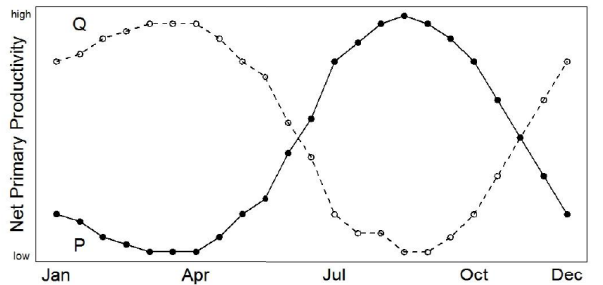
\includegraphics[]{figs/14.png}
    \caption{}
    \label{fig;1}
\end{figure}


\begin{enumerate}[nosep]

\item Habitat P is in Argentina while Q is in Canada
\item Habitat P is in Russia while Q is in Canada
\item Habitat P is in Russia while Q is in South Africa
\item Habitat P is in South Africa while Q is in Argentina
\end{enumerate}


\end{enumerate}
\hfill{(GATE EY 2019)}


\begin{enumerate}[resume]
%15
\item Which of the following statements best explains the patterns of leaf-litter decomposition over time shown in the figure below?

\begin{figure}[H]
    \centering
    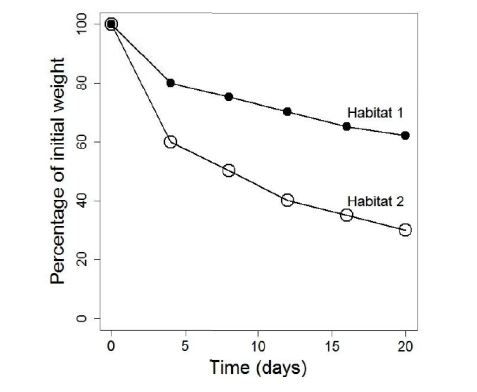
\includegraphics[]{figs/15.png}
    \caption{}
    \label{fig:2}
\end{figure}

\begin{enumerate}[nosep]
\item Habitat 1 is cold and wet; Habitat 2 is warm and arid
\item Habitat 1 is warm and arid; Habitat 2 is cold and wet
\item Habitat 1 is cold and arid; Habitat 2 is warm and wet
\item Habitat 1 is warm and wet; Habitat 2 is cold and arid
\end{enumerate}
\hfill{(GATE EY 2019)}
%16
\item To compare biomass of a fish species in two lakes, A and B, a researcher records live-weights of 30 individuals from each lake. She assumes that these two datasets are normally distributed and have equal variance. She calculates
\[
Q=\frac{\bar{x}_A-\bar{x}_B}{s}
\]
where $\bar{x}_A$ and $\bar{x}_B$ are mean values from the respective lakes, and $s$ is the pooled standard error.  

What is this quantity $Q$?
\begin{enumerate}[nosep]
\item Correlation coefficient
\item Regression coefficient
\item $t$-statistic
\item $\chi^2$-statistic
\end{enumerate}
\hfill{(GATE EY 2019)}

\end{enumerate}

%17
\begin{enumerate}[resume]

\item While developing his theory of evolution by natural selection, Charles Darwin was influenced by the work of  
\begin{multicols}{2}
\begin{enumerate}
\item Charles Lyell and Thomas Malthus  
\item Francis Crick and James Watson  
\item Gregor Mendel and J.B.S. Haldane  
\item Sewall Wright and Ronald Fisher  
\end{enumerate}
\end{multicols}
\hfill{(GATE EY 2019)}
%18
\item Weakly-electric fish typically produce electric voltages of less than 1 volt for communication and navigation. Which of the following features is NOT a characteristic of weakly-electric fish?  
\begin{multicols}{2}
\begin{enumerate}
\item Electrocytes  
\item Electrolocation capabilities  
\item Exclusively marine habit  
\item Mechanisms to avoid signal jamming  
\end{enumerate}
\end{multicols}
\hfill{(GATE EY 2019)}
%!9
\item Match the combination of primates and trees to the state/union territory where they can be found.  

\begin{center}
\begin{tabular}{|l|l|}
\hline
\textbf{Primate and Tree combination} & \textbf{State} \\
\hline
P: Bonnet macaque; Figs & i: Andaman and Nicobar Islands \\
Q: Crab-eating macaque; Mangroves & ii: Himachal Pradesh \\
R: Lion-tailed macaque; Myristica & iii: Maharashtra \\
S: Rhesus macaque; Deodar & iv: Kerala \\
\hline
\end{tabular}
\end{center}

\begin{multicols}{2}
\begin{enumerate}
\item P = i; Q = iii; R = iv; S = ii  
\item P = iii; Q = i; R = iv; S = ii  
\item P = ii; Q = i; R = iii; S = iv  
\item P = i; Q = iv; R = ii; S = iii  
\end{enumerate}
\end{multicols}
\hfill{(GATE EY 2019)}
%20
\item Which of the following crops should show the \textbf{LOWEST} proportional increase in photosynthetic rate under rising carbon dioxide levels in the atmosphere?  
\begin{multicols}{2}
\begin{enumerate}
\item Barley  
\item Maize  
\item Rice  
\item Wheat  
\end{enumerate}
\end{multicols}
\hfill{(GATE EY 2019)}
%21
\item Which among the following is the best indicator of the precision with which a population parameter is estimated?  
\begin{multicols}{2}
\begin{enumerate}
\item Degrees of freedom  
\item Mean  
\item Sample size  
\item Standard error  
\end{enumerate}
\end{multicols}

\end{enumerate}
\hfill{(GATE EY 2019)}
%22
\begin{enumerate}[resume]

\item Which of the following hormones regulates moulting in arthropods?  
\begin{multicols}{2}
\begin{enumerate}
\item Corticosterone  
\item Ecdysone  
\item Gibberellin  
\item Hydrocortisone  
\end{enumerate}
\end{multicols}
\hfill{(GATE EY 2019)}
%23
\item A study found that grazing decreased species richness when productivity was low, and increased species richness when productivity was high. Which of the following figures best represents this trend? In the figure, the dotted line represents species richness in grazed plots and the solid line represents species richness in plots without grazing.  


\begin{multicols}{2}
\begin{enumerate}
\item i  
\item ii  
\item iii  
\item iv  
\end{enumerate}
\end{multicols}
\hfill{(GATE EY 2019)}
%24
\item The mean height of students in a class (number of students, n=10) was initially estimated to be 6 feet and 6 inches. Later an error was detected, where one boy's height was recorded as 10 feet taller than his actual height. The correct mean height of the students in the class is\underline{\hspace{1.5cm}} inches (round off to 1 decimal place).
\end{enumerate}
\hfill{(GATE EY 2019)}



\begin{enumerate}[resume]
%25
\item Two true-breeding lines of a moth, one with black wings and the other with red wings, are crossed. All of the resulting offspring in the F$_1$ generation had red wings. These offspring are crossed to produce the F$_2$ generation of moths where the expected fraction of moths with black wings in the population is \underline{\hspace{1.5cm}}  (round off to two decimal places).
\hfill{(GATE EY 2019)}
\end{enumerate}


\textbf{Q.26-Q.55 carry two marks each}
\begin{enumerate}[resume]
%26
\item A teacher proposed a null hypothesis (H$_0$) that there is no difference in the mean heights of boys and girls in his class. His alternative hypothesis (H$_a$) was that boys are taller than girls.  

The figure below shows the probability distribution, i.e. probability density function, of the difference in the mean height of boys and girls if the null hypothesis were true. The observed mean difference in heights is shown by the solid black circle. The dotted line represents the range $\mu \pm 2\sigma$ whereas the solid line shows the range $\mu \pm 3\sigma$.  


Assuming a significance level of 0.05, which of the following conclusions is correct? 
\begin{figure}[h]
    \centering
    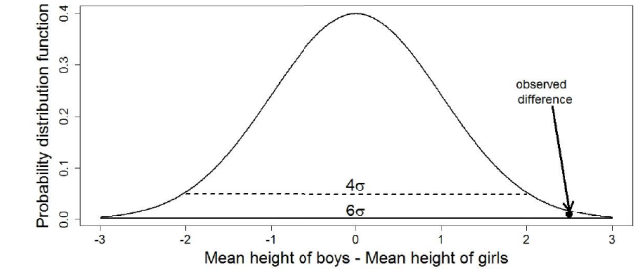
\includegraphics[]{figs/26.png}
    \caption{}
    \label{fig:3}
\end{figure}

\begin{multicols}{2}
\begin{enumerate}
\item H$_0$ is accepted
\item H$_0$ is rejected
\item H$_a$ is accepted
\item H$_a$ is rejected
\end{enumerate}
\end{multicols}

\hfill{(GATE EY 2019)}
%27
\item Females in many birds and mammals mate with multiple males, in addition to their paired-male. Which of the following is an \textbf{INCORRECT} adaptive explanation for such extra-pair mating?  
\begin{multicols}{2}
\begin{enumerate}
\item   Increased genetic quality of offspring
\item   Increased care of offspring by the paired-male
\item   Increased probability of fertilisation
\item   Increased resources for offspring production
\end{enumerate}
\end{multicols}


\end{enumerate}
\hfill{(GATE EY 2019)}
%28
\begin{enumerate}[resume]

\item A researcher hypothesized that females of a bird species prefer to mate with long-tailed males. To test this hypothesis, she assigned male birds of similar tail lengths to one of the following four treatments:  

 Intact -tails left unmanipulated  
 Re-attached - tails cut and re-attached without any change in length  
 Shortened - tails cut, shortened and re-attached  
 Elongated - tails cut, elongated and re-attached  

She measured mating success of these experimental birds and the results from this are shown below. Error bars represent 95\% confidence intervals. Which of the following inferences are consistent with these results?  


\begin{figure}[h]
    \centering
    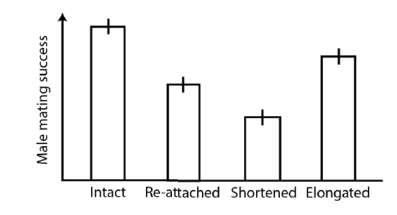
\includegraphics[]{figs/28.png}
    \caption{}
    \label{fig:4}
\end{figure}

i. Experimental manipulation of tails decreased male mating success  
ii. Females preferred to mate with males with short tails  
iii. Females preferred to mate with males with long tails  
\begin{multicols}{2}
\begin{enumerate}
\item   i only
\item   i and iii only
\item   i and ii only
\item   iii only
\end{enumerate}
\end{multicols}


\hfill{(GATE EY 2019)}
%29
\item Highly repetitive sequences are most likely to be prevalent in regions of the genome with  \underline{\hspace{1.5cm}}recombination rate and originate via  \underline{\hspace{1.5cm}}crossing over. Choose the right pair of words that completes this statement correctly.  
\begin{multicols}{2}
\begin{enumerate}
\item high; equal
\item high; unequal
\item low; equal 
\item low; unequal
\end{enumerate}
\end{multicols}

\hfill{(GATE EY 2019)}


\end{enumerate}
%30
\begin{enumerate}[resume]

\item Which of the following is correct about first and second derivatives at points P, Q and R for $f(x) = \sin(x)$ shown below?  
\begin{figure}[H]
    \centering
    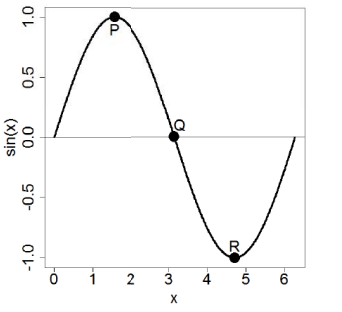
\includegraphics[]{figs/30.png}
    \caption{}
    \label{fig:5}
\end{figure}


\begin{enumerate}
\item  $\frac{df}{dx}\Big|_P = 0;\; \frac{d^2f}{dx^2}\Big|_P < 0;\; \frac{df}{dx}\Big|_Q < 0;\; \frac{d^2f}{dx^2}\Big|_Q = 0;\; \frac{df}{dx}\Big|_R = 0$
\item    $\frac{df}{dx}\Big|_P < 0;\; \frac{d^2f}{dx^2}\Big|_P < 0;\; \frac{df}{dx}\Big|_Q > 0;\; \frac{d^2f}{dx^2}\Big|_Q = 0;\; \frac{df}{dx}\Big|_R = 0$ 
\item  $\frac{df}{dx}\Big|_P < 0;\; \frac{d^2f}{dx^2}\Big|_P < 0;\; \frac{df}{dx}\Big|_Q < 0;\; \frac{d^2f}{dx^2}\Big|_Q > 0;\; \frac{df}{dx}\Big|_R = 0$
\item$\frac{df}{dx}\Big|_P = 0;\; \frac{d^2f}{dx^2}\Big|_P < 0;\; \frac{df}{dx}\Big|_Q < 0;\; \frac{d^2f}{dx^2}\Big|_Q > 0;\; \frac{df}{dx}\Big|_R = 0$
\end{enumerate}



\hfill{(GATE EY 2019)}
%31
\item Which of the following is NOT a proximate explanation for group cohesion among animals?  

\begin{enumerate}
   
\item Animals follow a common path while foraging 
\item Animals follow their nearest neighbor while foraging   
\item Animals reduce predation while foraging   
\item Animals secrete pheromones to attract conspecifics while foraging 
  
\end{enumerate}

 

\hfill{(GATE EY 2019)}
%32
\item Which of the following statements is LEAST likely to explain the evolution of dispersal?  

\begin{enumerate}
 
\item Dispersal enhances chances of finding novel habitats 
\item  Dispersal regulates population densities
\item  Dispersal reduces parent-offspring conflict   
\item Dispersal reduces sibling conflict 

\end{enumerate}


\hfill{(GATE EY 2019)}
%33
\end{enumerate}
\begin{enumerate}
\setcounter{enumi}{32}

\item Which of the following plots describes the expected relationship between population size (y-axis) and generation time (x-axis) in vertebrates? Here, each data point represents a different vertebrate species and the generation time is defined as the average interval between two generations.
\begin{figure}[h]
    \centering
    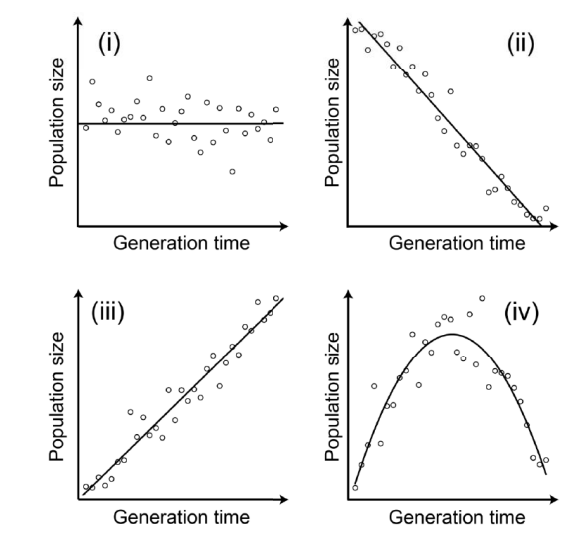
\includegraphics[]{figs/33.png}
    \caption{}
    \label{fig:6}
\end{figure}


\begin{multicols}{4}
\begin{enumerate}
\item i
\item ii
\item iii
\item iv
\end{enumerate}
\end{multicols}

\hfill{(GATE EY 2019)}
%34
\item Six different species of centipedes represented by the following phylogenetic tree have these single nucleotide polymorphisms (SNPs) at a given locus. Assuming maximum parsimony (or minimum evolutionary changes), what is the most likely nucleotide in the ancestor 'P'?
\begin{figure}[H]
    \centering
    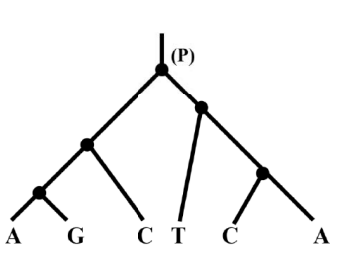
\includegraphics[]{figs/34.png}
    \caption{}
    \label{fig:7}
\end{figure}

\begin{multicols}{2}
\begin{enumerate}
\item A or C
\item A or G
\item C or G
\item C or T
\end{enumerate}
\end{multicols}
\hfill{(GATE EY 2019)}

%35
\item Garter snakes have evolved resistance to the poisonous secretions of the rough-skinned newts. The following figure describes poison production in newts and the resistance (measured as amount of poison tolerated) in garter snakes in three different geographical areas. Given this information, which of the following statements is correct regarding the evolution of poison resistance in garter snakes?
\begin{figure}[h]
    \centering
    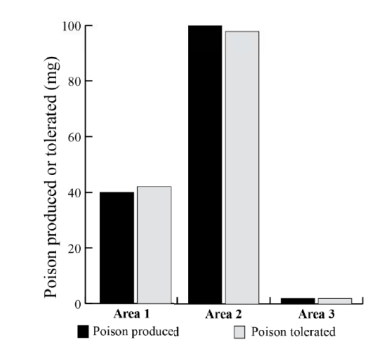
\includegraphics[]{figs/35.png}
    \caption{}
    \label{fig:8`}
\end{figure}

\begin{multicols}{2}
\begin{enumerate}
\item Evolution of resistance is neutral
\item Snakes in Area 2 are more adapted than the others
\item Snakes in Area 3 are less adapted than the others
\item The resistance mechanism is costly
\end{enumerate}
\end{multicols}
\hfill{(GATE EY 2019)}
%36
\item Many bird species show cooperative breeding. Offspring are cared for by parents and other individuals (helpers) who are typically offspring from previous years. Which of the following is NOT an appropriate evolutionary explanation for why helpers do not leave and breed on their own?

\begin{enumerate}
\item At high population density new breeding territories are difficult to obtain and helpers gain more from staying and helping than from dispersing to breed
\item In environments where resources are scarce, helpers gain more by suppressing their reproduction and minimizing population extinction than from dispersing to breed
\item When complex parental care is required for offspring survival, helpers gain more by staying and learning to care than from dispersing to breed
\item When predation risk during dispersal is high, helpers gain more by staying and helping than from dispersing to breed
\end{enumerate}


\hfill{(GATE EY 2019)}
%37


\item The relative performance of amphibians adapted to tropical (dashed line) and temperate (solid line) climates as a function of temperature is shown below. Assume that global warming will result in an equal increase in mean temperatures over the next 30 years in both regions. Which of the following statements about the effects of global warming on these two amphibians is most likely?
\begin{figure}[H]
    \centering
    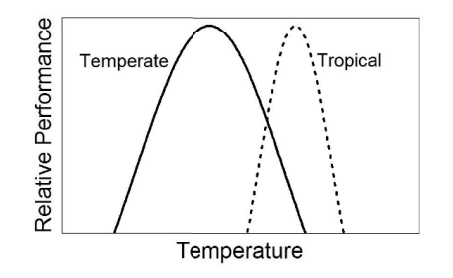
\includegraphics[]{figs/37.png}
    \caption{}
    \label{fig:9}
\end{figure}

\begin{enumerate}
\item Temperate and tropical amphibians will be similarly impacted
\item Temperate amphibians will be more negatively impacted than tropical amphibians
\item Tropical amphibians will be more negatively impacted than temperate amphibians
\item Tropical amphibians will be positively impacted, while temperate amphibians will be negatively impacted
\end{enumerate}


\hfill{(GATE EY 2019)}
%38
\item Global warming potential of different greenhouse gases (CO$_2$, CH$_4$, N$_2$O, etc) is determined by their:
\begin{enumerate}
\item P: ability to absorb infrared radiation
\item Q: concentration in the atmosphere
\item R: residence time in the atmosphere
\item S: source of origin (whether natural, or anthropogenic)
\end{enumerate}
 

\begin{multicols}{2}
\begin{enumerate}
\item P \& R only
\item P, Q \& R only
\item Q, R \& S only
\item Q \& S only
\end{enumerate}
\end{multicols}
\end{enumerate}
\hfill{(GATE EY 2019)}


\begin{enumerate}[resume]
%39
\item A hornbill foraging exclusively on figs in a tropical forest spends an average of 36 minutes on a tree before moving to the next tree. The density of fig trees in the forest decreases by half. In accordance with optimal foraging theory, which of following represents a possible duration (in minutes) that the hornbill may spend per tree?

\begin{multicols}{2}
\begin{enumerate}
\item 6
\item 18
\item 36
\item 54
\end{enumerate}
\end{multicols}
\hfill{(GATE EY 2019)}
%40
\item Type-I errors in statistical tests represent false positives, where a true null hypothesis is falsely rejected. Type-II errors represent false negatives where we fail to reject a false null hypothesis. For a given experimental system, increasing sample size will

\begin{multicols}{2}
\begin{enumerate}
\item decrease both Type-I and Type-II errors
\item decrease Type-I and increase Type-II errors
\item increase both Type-I and Type-II errors
\item increase Type-I and decrease Type-II errors
\end{enumerate}
\end{multicols}

\hfill{(GATE EY 2019)}
%41
\item Semelparous species are those that produce all of their offspring in a single reproductive event. The survivorship curve of a population of a semelparous species would most likely resemble which of the following?
\begin{figure}[H]
    \centering
    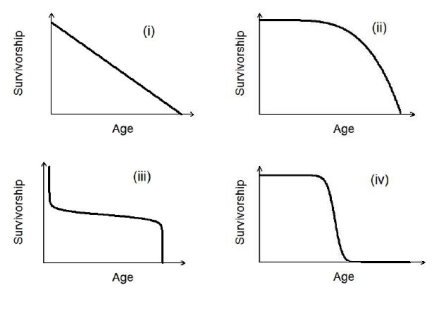
\includegraphics[]{figs/41.png}
    \caption{fig:10}
\end{figure}

\begin{multicols}{4}
\begin{enumerate}
\item i
\item ii
\item iii
\item iv
\end{enumerate}
\end{multicols}

\hfill{(GATE EY 2019)}

%42

\item Bergmanns rule describes the increase in body size observed in related organisms as we go from the equator to the poles. Which of the following is a possible explanation for this pattern?


\begin{enumerate}
\item Decreased body mass in smaller organisms helps generate less heat
\item Decreased surface area to volume ratios in larger organisms helps conserve heat
\item Increased body mass in the poles is necessary to counter increased competition
\item Increased surface area in larger organisms helps efficient gas exchange in the poles
\end{enumerate}


\hfill{(GATE EY 2019)}
%43
\item To estimate the number of foxes in an area, a researcher conducted a mark-recapture survey. In the first survey, he caught and marked 90 foxes. In his second survey a week later, he caught 120 foxes of which 40 were marked (recaptures). If you are told that the actual number of foxes in this area is 400, which of the following is a plausible explanation for the anomaly in the researcher's data?

\begin{enumerate}
\item Capture increased mortality in the marked foxes
\item Large mortality of foxes between the two surveys
\item The marked foxes were more likely to avoid recapture
\item The marked foxes were more likely to be recaptured
\end{enumerate}
\hfill{(GATE EY 2019)}
%44

\item Which one of the statements below best describes a plant species with the timing of reproductive events shown in the following figure?
\begin{figure}[H]
    \centering
    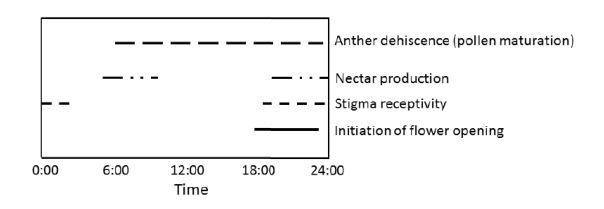
\includegraphics[]{figs/44.png}
    \caption{}
    \label{fig:11}
\end{figure}

\begin{enumerate}
\item The plant does not require animal pollinators
\item The plant relies on diurnal pollinators only
\item The plant relies on diurnal and nocturnal pollinators
\item The plant relies on nocturnal pollinators only
\end{enumerate}


\hfill{(GATE EY 2019)}
%45

\item Match species in column A to its phylogenetically closest relative in column B.

\begin{multicols}{2}
\textbf{Column A}\\
(P) Sperm whale\\
(Q) Corals\\
(R) Platypus\\
(S) Sea hare\\
(T) Prairie dog\\

\columnbreak

\textbf{Column B}\\
(W) Sea anemone\\
(X) Guinea Pig\\
(Y) Cuttlefish\\
(Z) Hippopotamus\\
(V) Echidna\\
\end{multicols}

\begin{multicols}{2}
\begin{enumerate}
\item P - W; Q - Y; R - Z; S - X; T - Y
\item P - W; Q - X; R - Z; S - X; T - Y
\item P - Y; Q - V; R - Z; S - W; T - X
\item P - Y; Q - X; R - Z; S - W; T - X
\end{enumerate}
\end{multicols}
\hfill{(GATE EY 2019)}
%46
\item Under which of the following conditions is rapid pollen tubes growth most likely to evolve?


\begin{enumerate}
\item In a self-compatible species with few ovules
\item In a self-compatible species with many ovules
\item In a self-incompatible species with few ovules
\item In a self-incompatible species with many ovules
\end{enumerate}

\hfill{(GATE EY 2019)}
%47
\item Which of the following correctly represents a decreasing order of tree species richness?  
P - Dry tropical forests in Maharashtra  
Q  - Lowland wet tropical forests in Arunachal Pradesh  
R - Scrub forest in Rajasthan  
S  - Wet tropical forests in Kerala

\begin{multicols}{2}
\begin{enumerate}
\item $Q > R > S > P$
\item $Q > S > P > R$
\item $S > P > Q > R$
\item $S > Q > R > P$
\end{enumerate}
\end{multicols}
\hfill{(GATE EY 2019)}

%48

\item A forester, pictured below, is trying to measure the height of a tree. Her height is $x=1.5$ m. She stands $y=10$ m away from a tree, from where the angle subtended to the top of the tree is $z=45^\circ$. The height of the tree is \underline{\hspace{1.5cm}} m (round off to 1 decimal place).

\begin{figure}[H]
    \centering
    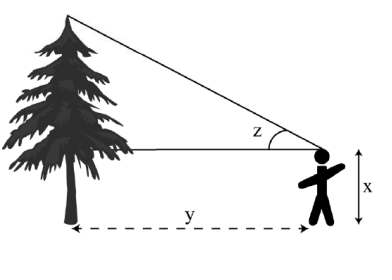
\includegraphics[]{figs/48.png}
    \caption{}
    \label{fig:12}
\end{figure}

\hfill{(GATE EY 2019)}
%49
\item In a recently discovered fossil, only 0.39\% of $^{14}C$ found in living fossils is present. If the half-life of $^{14}C$ is 5730 years, the age of the fossil is expected to be\underline{\hspace{1.5cm}} years (round off to the nearest integer).
\hfill{(GATE EY 2019)}

\item A beaker contains a large number of spherical nuts of two types, one with radius 1 cm and the other with 2 cm, in the ratio 2:1. A squirrel picks one nut from a random point in this beaker. Assuming that the beaker is well-mixed, the probability of picking the smaller nut is \underline{\hspace{1.5cm}} (round off to 1 decimal place).
\hfill{(GATE EY 2019)}
%50
\item In a closed population following logistic growth, per capita birth rate $b$ and per capita death rate $d$ vary with population size $N$ as $b=0.1-0.00001N$ and $d=0.01+0.00002N$, respectively. The carrying capacity $K$ of this population is\underline{\hspace{1.5cm}}individuals.
\hfill{(GATE EY 2019)}
%51
\item A population of birds has a 3:2 male to female adult sex ratio at the beginning of the breeding season. During the breeding season, every female produces 8 eggs of which 4 survive to become juveniles. A census at the end of the breeding season accurately estimates the bird population to be 1300 individuals. Assuming no deaths, the number of adult males in this population is \underline{\hspace{1.5cm}} individuals.
\hfill{(GATE EY 2019)}
%52
\item The coordinates of P is (0,1), Q is (0,3), R is (2,0) and S is (1,0). The area of the trapezoid PQRS is\underline{\hspace{1.5cm}} (round off to 1 decimal place).

\hfill{(GATE EY 2019)}
%53
\item Trees in two patches A and B can disperse seeds to a bare patch C. The probability of a seed being dispersed from A to C is 0.5 and the probability of germination of such a seed is 0.1. Likewise, the probability of a seed being dispersed from B to C is 0.4 and the probability of germination of such a seed is 0.2. If the number of seeds produced in patch A is 100 and that in B is 200, the expected number of germinated seeds in patch C is \underline{\hspace{1.5cm}}.
\hfill{(GATE EY 2019)}
\begin{figure}[H]
    \centering
    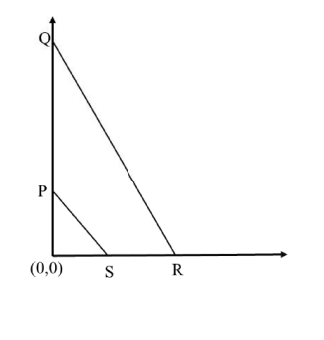
\includegraphics[]{figs/53.png}
    \caption{fig:13}
    \label{}
\end{figure}
%54

\item A bacterial population grows from $10^6$ cells to $5.5 \times 10^7$ cells in 20 minutes. Assuming that the growth was not resource limited, the per-capita growth rate of bacteria is \underline{\hspace{1.5cm}}per minute (round off to 2 decimal places).
\hfill{(GATE EY 2019)}

\begin{center}
    \textbf{END OF THE QUESTION PAPER}
\end{center}
\end{enumerate}


\end{document}

